\documentclass[12pt]{article}

\input preamble

\title{Principles of Parallel Architecture\\
Project Report 1}
\author{Xitong Liu \\
xliu@ece.udel.edu}

\begin{document}

\maketitle

\section{Project Description}
The class project is designed to explore and understand a 
particular aspect of parallel architecture and parallel 
computing.

We choose Matrix Multiply as the topic of my project and use 
OpenMP to implement parallel computation.

\section{Implementation}
The intuitive way to implement matrix multiplication in a 
parallel is to divide the matrix evenly into several
sub-matrices. The details is shown in 
Fig.\ref{fig:matrix-divide}, in which we divide Matrix A
evenly into several parts, and each thread will try to 
calculate the associated sub-part of results in Matrix C.

\begin{figure}[h!]
	\begin{center}
		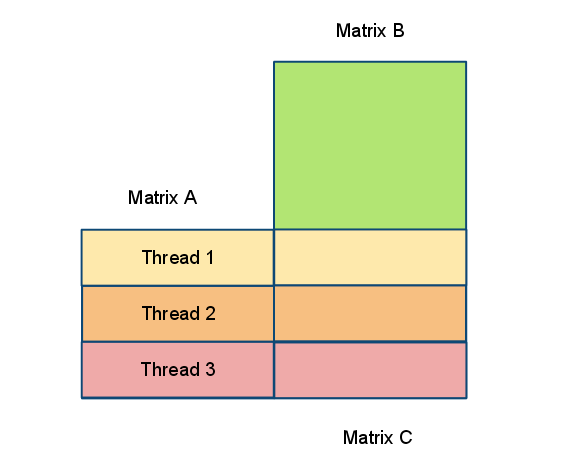
\includegraphics[width=0.5\textwidth]{matrix-divide.png}
		\caption{\label{fig:matrix-divide}Divide the matrix 
			evenly by the number of threads}
	\end{center}
\end{figure}

To make sure the data is distributed evenly in the threads, 
I made a division on the matrix size. For example, if the 
matrix size is $77\times 77$ and the number of threads is 
8, it will be divided in the following way. $77 = 8\times 9+5$, 
so each thread will calculate at least 9 rows of data. 
For the remainder 5, it will distributed evenly in the first 
5 threads. Thus, $79=8\times 9+5 = 5\times 10+3\times 9$. 
More specifically, thread \#0 to \#4 will calculate 10 rows 
and others will calculate 9 rows.

\small
\begin{verbatim}
  // calculate the sum in parallel
  omp_set_num_threads(thread_num);
#pragma omp parallel private (thread_id) shared (matrixC)
  {
    int num_per_thread = 0;
    int remainder = 0;
    int range_start = 0;
    int range_end = 0;
    int range_len = 0;

    // get the thread id
    thread_id = omp_get_thread_num();
    
    // Make sure the data is evenly distributed between the processes
    num_per_thread = dim / thread_num;
    remainder = dim % thread_num;
    if(0 == remainder){
      range_start = thread_id * num_per_thread;
    }else{
      range_start = thread_id * (num_per_thread + 1);
      range_start = (thread_id > remainder) ? 
        range_start - thread_id + remainder : range_start;
    }
    range_end = (thread_id > remainder - 1) ? 
      range_start + num_per_thread : range_start + num_per_thread + 1;
    range_len = range_end - range_start;

    int cycleI = 0;
    int cycleJ = 0;
    int cycleK = 0;

    for(cycleI = range_start; cycleI < range_end; ++ cycleI){
      for(cycleJ = 0; cycleJ < matrixB.xDim; ++ cycleJ){

        matrixC.data[cycleI * dim + cycleJ] = 0.0;

        for(cycleK = 0; cycleK < dim; ++ cycleK){
          matrixC.data[cycleI * dim + cycleJ] += 
            matrixA.data[cycleI * matrixA.xDim + cycleK] *
            matrixB.data[cycleJ + cycleK * matrixB.xDim];
        }

      }
    }
  }
\end{verbatim}
\normalsize
\section{Performance Evaluation}
\subsection{Speed}
The Time vs problem size graph is shown is Fig.\ref{fig:speed}.
\begin{figure}[h!]
	\begin{center}
		\includegraphics[width=0.6\textwidth, angle=0]{speed.pdf}
		\caption{\label{fig:speed}Time vs Problem size.}
	\end{center}
\end{figure}

\subsection{Speedup}
The Speedup vs problem size graph is shown is Fig.\ref{fig:speedup}.
\begin{figure}[h!]
	\begin{center}
		\includegraphics[width=0.6\textwidth, angle=0]{speedup.pdf}
		\caption{\label{fig:speedup}Speedup vs Problem size.}
	\end{center}
\end{figure}

Obviously, when the problem is small ( $N \le 200$ ), the speedup 
is less than 1, which means that the overhead for parallel program 
overwhelmed the benefit. When the problem get greater, the speedup
increases and is greater than 1. However, it stop growth when the 
problem size reaches 800. 

\subsection{Memory Usage}
Since we need two matrices to hold the operands for 
multiplication, two matrices to hold the results, one for 
parallel computation and the other for serial computation, 
respectively. Hence the total memory usage given by the 
problem size $N$ is $4N^{2}$.

\section{Result Validation}
To validate the correctness of our results, we provided a serial
implementation of matrix multiplication. After the parallel 
computation is complete, we will do the serial computation and
compare the results of them. The input data for parallel 
computation are the same as that for serial computation, so if 
the results for them are the same, it's a strong proof that 
the parallel computation is correct.

\end{document}

\begin{comment}
\begin{figure}[h!]
	\begin{center}
		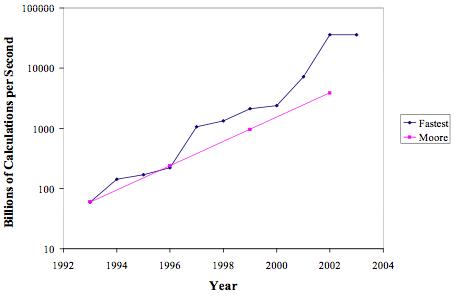
\includegraphics[width=0.7\textwidth, angle=0]{fatest.png}
		\caption{\label{fig:fatest}Fatest SuperComputer in the world}
	\end{center}
\end{figure}
\end{comment}